\documentclass[../../main]{subfiles}
\pagestyle{fancy}

\begin{document}

\chapter{Preliminaries}
\thispagestyle{fancy}

This chapter will give a rough overview of concepts that will be used in subsequent chapters. We start with briefly recalling properties regarding filters and elementary embeddings that we will be employing, as well as describing \gbc\, G\"odel-Bernays class theory. We then spend some time on large cardinal theory, as it plays a prominent role in understanding how the \textit{virtual} large cardinals in Chapter~\ref{chapter.virtual-large-cardinals} compares to the other large cardinals.

We will also routinely be working with the core model $K$ throughout this thesis, so we include a section that will give a high-level overview of what $K$ is and which key properties it has. The last section in these preliminaries will cover some results related to working with elementary embeddings in different forcing extensions, which tend to not be covered in standard textbooks. In the interest of brevity we will provide references rather than proofs of most of these results.


\section{Filters and elementary embeddings}
\label{prelims.filters}

When we are dealing with elementary embeddings between set-sized structures, we will usually be interested in structures of the following form:

\defi{
	For a cardinal $\kappa$, a \textbf{weak $\kappa$-model} is a set $\M$ of size $\kappa$ satisfying that $\kappa+1\subset\M$ and $(\M,\in)\models\zfc^-$. If furthermore $\M^{<\kappa}\subset \M$, $\M$ is a \textbf{$\kappa$-model}.\footnote{Note that our (weak) $\kappa$-models do not have to be transitive, in contrast to the models considered in \cite{Ramsey1} and \cite{Ramsey2}. Not requiring the models to be transitive was introduced in \cite{HolySchlicht}.}
}

A proto-typical example of a weak $\kappa$-model is any $\kappa$-sized $M\prec H_{\kappa^+}$, as it is well-known that $H_{\kappa^+}$ satisfies $\zfc^-$. We can get a $\kappa$-model from this by closing off $M$ under ${<}\kappa$-sequences while maintaining being an elementary substructure of $H_{\kappa^+}$. Note that this only works if $2^{<\kappa}=\kappa$ however, as otherwise the resulting structure would be too large.

Embeddings between these weak $\kappa$-models can equivalently be phrased in terms of ultrafilters, or \textit{measures}. Recall that $\mu$ is an \textbf{$\M$-measure} if
\eq{
  (\M,\in,\mu)\models\godel{\mu\text{ is a $\kappa$-complete ultrafilter on $\kappa$}}.
}

Some common properties of such measures are the following:

\xdefi{
	For a weak $\kappa$-model $\M$, an $\M$-measure $\mu$ is...
\begin{itemize}
	\item \textbf{weakly amenable} if $x\cap\mu\in\M$ for every $x\in\M$ with $\Card^{\M}(x)=\kappa$;
	\item \textbf{countably complete} if $\bigcap\vec X\neq\emptyset$ for every $\omega$-sequence $\vec X\in{^\omega\mu}$.$\hfill\circ$
\end{itemize}
}

Weak amenability can equivalently be phrased in terms of a property concerning only the embedding.

\qprop[\cite{KunenPhD}]{
	Let $\M$ be a weak $\kappa$-model, $\mu$ an $\M$-measure and $j:\M\to\N$ the ultrapower embedding. Then $\mu$ is weakly amenable iff $j$ is \textbf{$\kappa$-powerset preserving}, meaning that $\M\cap\p(\kappa)=\N\cap\p(\kappa)$.
}

We will also be employing the following well-known result regarding set-sized embeddings:

\lemm[Ancient Kunen Lemma][lemm.kunen]{
  Let $\kappa$ be regular, $\M,\N$ weak $\kappa$-models, $\theta\in(\kappa,o(\M))$ a regular $\M$-cardinal, and $\pi\colon\M\to\N$ an elementary embedding with $\crit\pi=\kappa$ and $H_\theta^{\M}\subset\N$. Then for every $X\in H_\theta^{\M}$ with $\card^{\M}(X)=\kappa$ it holds that $\pi\restr X\in\N$.
}
\proof{
  Let $f\colon\kappa\to X$, $f\in\M$, be a bijection and note that $\pi(x)=\pi(f)(f^{-1}(x))$ for all $x\in X$, so it suffices that $f,\pi(f)\in\N$, which is true since $f\in H_\theta^{\M}\subset\N$.
}



\section{G\"odel-Bernays class theory}
\label{prelims.gbc}

As we will often find ourselves working with proper classes, we need to be able to work rigourously with these. We formalise this in second-order \textit{G\"odel-Bernays class theory}, \gbc. In the following we will use the standard convention of using uppercase letters for classes and lowercase letters for sets.

\xdefi{
  The axioms of \textbf{G\"odel-Bernays set theory with Choice}, \gbc, are as follows.
  \begin{enumerate}
    \item \zfc;
    \item (Class extensionality) Two classes are equal iff they have the same elements;
    \item (Class replacement) Every class-sized function restricted to a set is a set;
    \item (Class comprehension scheme) For classes $Y_1,\dots,Y_m$ and every formula $\varphi(v_1,\dots,v_n,V_1,\dots,V_m)$ that only quantifies over sets it holds that
      \eq{
        \{(x_1,\dots,x_n)\mid\varphi[x_1,\dots,x_n,Y_1,\dots,Y_m]\}
      }
      
      is a class;
    \item (Global choice) There is a class function $G$ such that, for every non-empty set $x$, $G(x)\in x$.$\hfill\circ$
  \end{enumerate}
}

\qtheo[Cohen-Kripke-Solovay; \cite{Cohen-book}]{
  \gbc\ is \textit{conservative} over \zfc, meaning that if $\sigma$ is a first-order sentence and $\gbc\proves\sigma$ then $\zfc\proves\sigma$ as well. Intuitively speaking, \gbc\ does not add new information about sets.
}


\section{Large cardinals}
\label{prelims.large-cardinals}

Since large cardinals came into existence in the beginning of the 20th century, a vast zoo of different types of such have appeared. The aim of this section is to act as a reference for the definitions of these as well as the relations between them.

\qquad Large cardinals are roughly split into two ``sections'': the small ones and the large ones. This distinction is a bit blurry and varies from set theorist to set theorist, but here the distinction will be made at the point where \textit{global elementary embeddings} enter the picture, which starts at the measurable cardinals.

\qquad We will start from the bottom and only cover the large cardinals that we will be dealing with in this thesis. See Figure~\ref{fig.large-cardinals} for an overview of these.

\subsection{Small large cardinals}

The first large cardinal lies at the very bottom of the hierarchy: the inaccessibles.

\defi{
  A cardinal $\kappa$ is \textbf{regular} if $\cof\kappa=\kappa$; i.e. that there is no ordinal $\gamma<\kappa$ with a cofinal function $f\colon\gamma\to\kappa$. $\kappa$ is a \textbf{strong limit} if $2^\lambda<\kappa$ for all cardinals $\lambda<\kappa$. If $\kappa$ is both regular and a strong limit then we say that it is (strongly) \textbf{inaccessible}.
}

Every other large cardinal is either inaccessible or implies that there exists an inner model with an inaccessible cardinal. The following shows that inaccessible cardinals transcend \zfc:

\qprop[Sierpi\' nski-Tarski-Zermelo; \cite{Kanamori} 1.2]{
  If $\kappa$ is an inaccessible cardinal then $(V_\kappa, \in)\models\zfc$.
}

G\"odel's Second Incompleteness Theorem from \cite{godel-incompleteness} then shows that \zfc\ can prove neither the existence of any inaccessible cardinals nor the mere consistency of inaccessible cardinals existing. This is the foundation of the large cardinal hierarchy. We say that a large cardinal is \textbf{stronger} than another large cardinal if the former proves the consistency of the latter, so that the same application of the Incompleteness Theorem shows that the weaker large cardinal theory can never prove the consistency of the stronger one.

\qquad Taking a tiny step further, we arrive at the (inaccessible) $\Sigma_n$-reflecting cardinals.

\defi{
  For $n<\omega$, an inaccessible cardinal $\kappa$ is \textbf{$\Sigma_n$-reflecting} if it holds that $H_\kappa\prec_n V$.
}

Note that it is also common to not require inaccesibility of $\Sigma_n$-reflecting cardinals, in which case they are simply equiconsistent with $\zfc$ by the Reflection Theorem. But as all our $\Sigma_n$-reflecting cardinals will be inaccessible in this thesis we include this in the definition.

\prop[Folklore]{
  For $n\geq 2$, every $\Sigma_n$-reflecting cardinal is a limit of inaccessible cardinals.
}
\proof{
  Let $\kappa$ be $\Sigma_n$-reflecting. Note that the definitions of both regularity and strong limit are $\Pi_1$-formulae, making inaccessibility $\Pi_1$ as well. But now we get that, for every $\xi<\kappa$, $V\models\exists\lambda>\xi\colon\godel{\text{$\lambda$ is inaccessible}}$. This statement is a $\Sigma_2$-sentence, so since we in particular have that $H_\kappa\prec_2 V$ it holds that
  \eq{
    H_\kappa\models\exists\lambda>\xi\colon\godel{\text{$\lambda$ is inaccessible}}.
  }

  We can therefore define a sequence of inaccessible cardinals $\bra{\lambda_\alpha\mid\alpha<\kappa}$ with $\lambda_0$ being the least inaccessible below $\kappa$, $\lambda_{\alpha+1}$ being the least inaccessible cardinal in $(\lambda_\alpha,\kappa)$, and $\lambda_\gamma$ being the least inaccessible cardinal in $[\sup_{\alpha<\gamma}\lambda_\alpha,\kappa)$ for $\gamma<\kappa$ a limit ordinal. These exist by regularity of $\kappa$ and since a cardinal $\lambda<\kappa$ is inaccessible iff $H_\kappa\models\godel{\text{$\lambda$ is inaccessible}}$ by $\Sigma_1$-reflection.
}

\qquad Next, we move a handful of steps up the large hierarchy ladder and introduce the \textit{weakly compact cardinals}. These have a multitude of different equivalent definitions which we will not cover here, but instead define them in terms of a combinatorial colouring relation. We need a definition.

\defi[][defi.homogeneous]{
  For any function $f\colon A\to B$, a subset $H\subset A$ is \textbf{homogeneous for $f$} if $f\restr H$ is a constant function.
}

We may think of $f$ in the above Definition~\ref{defi.homogeneous} as being a \textit{colouring function} that colours elements of $A$ in colours taken from $B$. For $H\subset A$ to be homogeneous would then mean that everything in $H$ has the same colour.

\defi{
  An uncountable cardinal $\kappa$ is \textbf{weakly compact} if to every function $f\colon[\kappa]^2\to\{0, 1\}$ there is a $H\subset[\kappa]^2$ of size $\kappa$ which is homogeneous for $f$.
}

Again, thinking in terms of colourings, $\kappa$ is weakly compact if whenever we colour pairs of ordinals below $\kappa$ in two colours, then we can find a large (i.e. of size $\kappa$) set of such pairs all of the same colour.

\qquad The following result then shows that the weakly compact cardinals are indeed stronger than the inaccessibles:

\qtheo[Erd\H os-Tarski; \cite{Jech} 9.9]{
  Every weakly compact cardinal is a limit of inaccessible cardinals.
}

Moving a tiny step further, we introduce two strengthenings of the weakly compacts: the \textit{ineffables} and the \textit{completely ineffables}.

\defi{
  An uncountable cardinal $\kappa$ is \textbf{ineffable} if there to any function $f\colon[\kappa]^2\to~2$ exists a \textit{stationary} $H\subset[\kappa]^2$ which is homogeneous for $f$.
}

Ineffable cardinals are weakly compact by definition, and the following theorem from \cite{Friedman} shows that they are strictly stronger:

\qtheo[Friedman]{
  Ineffable cardinals are weakly compact limits of weakly compacts.
}

A way of improving ineffability is to ``close under homogeneity'', in the sense that if $H$ is homogeneous for $f\colon[\kappa]^2\to 2$ and $g\colon[H]^2\to 2$ is any function, then there is a subset of $H$ which is homogeneous for $g$. To formalise this notion we use the concept of a \textit{stationary class}.

\xdefi{
  For $X$ any set, a set $\R\subset\p(X)$ is a \textbf{stationary class} if
  \begin{itemize}
    \item $\R\neq\emptyset$;
    \item Every $A\in\R$ is a stationary subset of $X$;
    \item If $A\in\R$ and $B\supset A$ then $B\in\R$.$\hfill\circ$
  \end{itemize}
}

\defi{
  An uncountable cardinal $\kappa$ is \textbf{completely ineffable} if there is a stationary class $\R\subset\p(\kappa)$ such that for every $A\in\R$ and $f\colon[A]^2\to 2$ there exists a $H\in\R$ which is homogeneous for $f$.
}

As suspected, these completely ineffable cardinals are indeed strictly stronger than the ineffables, as the following theorem shows:

\qtheo[\cite{Abramson}]{
  Completely ineffable cardinals are ineffable limits of ineffable cardinals.
}

The next kind of large cardinal involves elementary embeddings. To motivate the definition we note the following characterisation of the weakly compact cardinals:

\qtheo[\cite{Hauser}]{
  An uncountable cardinal $\kappa$ is weakly compact if and only if for every $A\subset\kappa$ there exist weak $\kappa$-models $\M,\N$ with $A\in\M$ and an elementary embedding $\pi\colon\M\to\N$ with $\crit\pi=\kappa$.
}

We would arrive at a natural strengthening of this characterisation if we require more agreement between $\M$ and $\N$, leading to the following definition:

\defi[\cite{Ramsey1}]{
  An uncountable cardinal $\kappa$ is \textbf{1-iterable} if to every subset $A\subset\kappa$ there exists a weak $\kappa$-model $\M$ such that $A\in\M$ and there exists a weakly amenable $\M$-measure $\mu$ on $\kappa$ such that $\ult(\M,\mu)$ is wellfounded.
}

In the same paper, Gitman shows that these large cardinals are indeed consistency-wise stronger than the completely ineffables.

\qtheo[\cite{Ramsey1}]{
  Every $1$-iterable cardinal is a limit of completely ineffable cardinals.
}

Lastly, the \textit{Ramsey cardinals} are natural strengthenings of the weakly compacts.

\defi{
  An uncountable cardinal $\kappa$ is \textbf{Ramsey} if there to every function $f\colon[\kappa]^{<\omega}\to\{0,1\}$ exists a subset $H\subset[\kappa]^{<\omega}$ such that, for every $n<\omega$, $H\cap[\kappa]^n$ is homogeneous for $f\restr[\kappa]^n$.
}

See Figure~\ref{fig.large-cardinals} for an overview of all the large cardinals covered in this section.

\subsection{Large large cardinals}

Moving on to the higher reaches of the large cardinals, these are more uniformly defined and all involve elementary embeddings. Our first type of large large cardinal is the measurable cardinal, being the first cardinal witnessing an elementary embedding from the entire universe. We formalise this in \gbc, defined in Section \ref{prelims.gbc}.

\defi[\gbc]{
  An uncountable cardinal $\kappa$ is \textbf{measurable} if there exists a transitive class $\M$ and an elementary embedding $j\colon (V,\in)\to(\M,\in)$ with critical point $\kappa$.
}

The measurable cardinals were the first cardinals shown to ``transcend'' G\"odel's constructible universe $L$.\footnote{For more information about $L$, see e.g. \cite{SchindlerBook}} This was proven by Dana Scott and has now become known as Scott's Theorem.\footnote{The measurables are not the weakest large cardinals with this property, however. For instance, the Ramsey cardinals enjoy this property too, but none of the other large cardinals described in the previous subsection enjoys this property.}

\qtheo[Scott's Theorem; \cite{Kanamori} 5.5][theo.scott]{
  $L$, G\"odel's constructible universe, has no measurable cardinals.
}

Given this result, it is not surprising that the measurables then exceed the strength of the previous large cardinals.

\prop{
  Measurable cardinals are completely ineffable limits of completely ineffable cardinals.
}
\proof{
  (Sketch) If $j\colon V\to\M$ is a non-trivial elementary embedding then the \textbf{derived ultrafilter} $\mu\subset\p(\kappa)$ on $\kappa:=\crit j$ is defined as $X\in\mu$ iff $\kappa\in j(X)$. Section 5 in \cite{Kanamori} shows that it is indeed an ultrafilter and that its ultrapower $\ult(V, \mu)$ is wellfounded. A reflection argument then shows that we can simply take $\R:=\mu$.
}

Moving even further, we strengthen the definition of measurable cardinals to arrive at the \textit{strong cardinals}.

\defi[\gbc]{
  An uncountable cardinal $\kappa$ is \textbf{strong} if there to every cardinal $\theta>\kappa$ exists a transitive class $\M_\theta$ satisfying that $H_\theta\subset\M_\theta$, and an elementary $j_\theta\colon(V,\in)\to(\M_\theta,\in)$ with critical point $\kappa$. We say that $\kappa$ is \textbf{$\theta$-strong} if the property holds for a specific $\theta$.
}

\qprop[Gaifman, \cite{Kanamori} 26.6]{
  Strong cardinals are measurable limits of measurable cardinals.
}

One property of the strong cardinals that we will get back to in the next subsection and which will be important in Chapter \ref{chapter.virtual-large-cardinals} is the following:

\qprop[\cite{Kanamori} 26.7][prop.strong-prestrong-equivalence]{
  If $j\colon V\to\M_\theta$ witnesses that $\kappa:=~\crit j$ is a $\theta$-strong cardinal then $j(\kappa)>\theta$.
}

We can strengthen the strongs even more by requiring \textit{sequence closure} rather than only containing an initial segment of the universe.

\defi[\gbc]{
  An uncountable cardinal $\kappa$ is \textbf{supercompact} if there to every cardinal $\theta>\kappa$ exists a transitive class $\M_\theta$ satisfying that $^{<\theta}\M_\theta\subset\M_\theta$, and an elementary $j_\theta\colon(V,\in)\to(\M_\theta,\in)$ with critical point $\kappa$.
}

To get an intuition of why the sequence closure is a lot more powerful, note that bits of the elementary embedding itself are now elements of $\M_\theta$, so that $\M_\theta$ can now start reasoning about large cardinals and, $j_\theta$ being elementary, these facts will then be carried back into the universe. Here is an example of such an argument.

\prop{
  If $\kappa$ is supercompact then
  \eq{
    V_\kappa\models\godel{\text{There exists a proper class of strong cardinals}}.\tag*{$(1)$}
  }
}
\proof{
  (Sketch) By noting that the restrictions of the supercompact embedding is an element of the target model by supercompactness, $\kappa$ is strong up to $j(\kappa)$ in the target model, so that a reflection argument shows $(1)$.
}

\cite{Magidor-supercompact} introduced the following equivalent definition of supercompactness\footnote{See Theorem 22.10 in \cite{Kanamori} for a proof.}:

\defi{
  A cardinal $\kappa$ is supercompact iff for every regular $\theta>\kappa$ there is a $\bar\theta<\kappa$ and an elementary embedding $\pi\colon H_{\bar\theta}\to H_{\theta}$ with $\pi(\crit\pi)=\kappa$.
}

Another way of strengthening the strong cardinals is by restricting the behaviour of what the elementary embedding can do on certain sets.

\defi[][defi.A-strong]{
  Let $A$ be any (potentially proper) class. An uncountable cardinal $\kappa$ is \textbf{$A$-strong} if there to every cardinal $\theta>\kappa$ exists a transitive class $\M_\theta$ satisfying that $H_\theta\subset\M_\theta$, and an elementary $j_\theta\colon(V,\in)\to(\M_\theta,\in)$ with critical point $\kappa$, such that $A\cap H_\theta = j(A)\cap H_\theta$.\footnote{When $A$ is a proper class then $j(A)$ is short for the proper class $\bigcup_{\theta\in\on}j(A\cap H_\theta)$.}
}

These $A$-strong cardinals are not used much in practice, but the following \textit{Woodin cardinals} are immensely useful and can be seen as a ``local'' version of a proper class of $A$-strongs for every class $A$:

\defi{
  An uncountable cardinal $\delta$ is a \textbf{Woodin cardinal} if there to every subset $A\subset H_\delta$ exists a cardinal $\kappa<\delta$ such that $(H_\delta, \in, A)\models\godel{\text{$\kappa$ is $A$-strong}}$.
}

Woodin cardinals can equivalently be defined in terms of functions instead of the $A$-strong cardinals.

\theo[Woodin; \cite{Kanamori} 26.14]{
  The following are equivalent for an uncountable cardinal $\kappa$:
  \begin{enumerate}
    \item $\kappa$ is a Woodin cardinal;
    \item For any $f\colon\kappa\to\kappa$ there exists $\alpha<\kappa$ such that $f[\alpha]\subset\alpha$, a transitive $\M$ with $V_{j(f)(\alpha)}\subset\M$ and an elementary embedding $j\colon(V,\in)\to(\M,\in)$ with $\crit j=\kappa$.
  \end{enumerate}
}

Our last large cardinal in this section is ostensibly completely different from the others. It originates from category theory, and according to \cite{pudlak} was originally proposed by Petr Vop\v enka as a ``bogus large cardinal property'' which he believed was inconsistent with \zfc, but a proof of this never appeared.

\defi[\gbc]{
  \textbf{Vop\v enka's Principle (\vp)} postulates that to any first-order language $\mathcal L$ and proper class $\C$ of $\mathcal L$-structures, there exist distinct $\M,\N\in\C$ and an elementary embedding $j\colon\M\to\N$.
}

\defi{
  An uncountable cardinal $\delta$ is \textbf{Vop\v enka} if $(V_\delta,\in;V_{\delta+1})\models\vp$.
}

Perlmutter showed that the Woodin- and Vop\v enka cardinals are closely connected, with Woodin cardinals relating to Vop\v enka cardinals in the same way that strong cardinals relate to supercompacts.

\qtheo[\cite{Perlmutter}]{
  Vop\v enka cardinals are equivalent to cardinals $\delta$ that are ``Woodin for supercompactness'', meaning that to any subset $A\subset H_\delta$ there is a cardinal $\kappa<\delta$ with $(H_\delta,\in,A)\models\godel{\text{$\kappa$ is $A$-supercompact}}$.\footnote{Here $\kappa$ is, in analogy with Definition \ref{defi.A-strong}, \textbf{$A$-supercompact} if there to every cardinal $\theta>\kappa$ exists a transitive class $\M_\theta$, closed under ${<}\theta$-sequences, and an elementary $j_\theta\colon(V,\in)\to(\M_\theta,\in)$ with critical point $\kappa$, such that $A\cap H_\theta=j(A)\cap H_\theta$.}
}

See Figure~\ref{fig.large-cardinals} for an overview of all the large cardinals covered in this section.

\subsection{Inconsistent large cardinals}

In these highest reaches of the large cardinal hierarchy we encounter large cardinals whose existence are inconsistent with \zfc. The reason why these are still interesting to us is because none of them have yet been proven inconsistent with \zf. The first such cardinal is the following:

\defi[\gbc]{
  An uncountable cardinal $\kappa$ is a \textbf{Reinhardt cardinal} if there exists an elementary embedding $j\colon(V,\in)\to (V,\in)$ with $\crit j=\kappa$.
}

This was shown to be inconsistent in \cite{kunen-inconsistency}.

\theo[Kunen inconsistency; \gbc; \cite{Kanamori} 23.12]{
  There is no non-trivial elementary $j\colon(V_{\lambda+2},\in)\to(V_{\lambda+2}, \in)$ for any uncountable cardinal $\lambda$. In particular, there is no Reinhardt cardinal.
}

The proof of Proposition~\ref{prop.strong-prestrong-equivalence}, which stated that $j(\kappa)>\theta$ always holds for strong cardinals $\kappa$, relies heavily on the Kunen inconsistency. When we are going to deal with the \textit{virtual} large cardinals in Chapter \ref{chapter.virtual-large-cardinals} we do not have such a Kunen inconsistency and we will show that in that case the property $j(\kappa)>\theta$ is a highly non-trivial assumption.

\qquad There is also the following strengthening of the Reinhardts, in analogy with the strong cardinals:

\defi{
  An uncountable cardinal $\kappa$ is \textbf{super Reinhardt} if for all ordinals $\lambda$ there exists an elementary embedding $j\colon (V,\in)\to(V,\in)$ with $\crit j=\kappa$ and $j(\kappa)>\lambda$.
}

We can improve this even further by defining a notion corresponding to Woodin cardinals. If we define $\kappa$ to be \textbf{$A$-super Reinhardt} for a class $A$ to be a super Reinhardt cardinal with $\bigcup_{\alpha\in\on}j(A\cap V_\alpha)=A$, in analogy with the $A$-strong cardinals, then we define the \textit{totally Reinhardts} as follows.

\xdefi{
  An inaccessible cardinal $\kappa$ is \textbf{totally Reinhardt} if for each $A\subset V_\kappa$ it holds that
  \eq{
    (V_\kappa, \in; V_{\kappa+1})\models\godel{\text{There exists an $A$-super Reinhardt cardinal}}.\tag*{$\circ$}
  }
}

The last large cardinals that we will introduce are the Berkeley cardinals. These were introduced by Woodin at University of California, Berkeley around 1992. Similar to the Vop\v enka cardinals, these were introduced as a large cardinal candidate that would ``clearly'' be inconsistent with \zf, but such as result has not yet been found. They imply the Kunen inconsistency and are therefore at least inconsistent with \zfc, but that is as far as it currently goes.

\qquad We start with a preliminary definition.

\defi[\gb]{
  An uncountable cardinal $\delta$ is a \textbf{proto-Berkeley cardinal} if to every transitive \textit{set} $\M$ such that $\delta\subset\M$ there exists an elementary embedding $j\colon(\M,\in)\to(\M,\in)$ with $\crit j<\delta$.
}

To see that these indeed imply the Kunen inconsistency, note that we in particular get an elementary embedding $\pi\colon V_{\gamma + 2}\to V_{\gamma + 2}$, which is inconsistent by Corollary 23.14 in \cite{Kanamori}.

\qquad Note that if $\kappa$ is a proto-Berkeley cardinal then every $\lambda>\kappa$ is also proto-Berkeley, which makes it quite an uninteresting notion. But we can isolate the interesting cases, leading to the definition of a Berkeley cardinal. 

\qtheo[\cite{Cutolo} 2.1.14]{
  If $\delta_0$ is the least proto-Berkeley cardinal then we can choose the critical point of the embedding to be arbitrarily large below $\delta_0$.
}

As this property is clearly not preserved upwards, this makes for a good candidate for the large cardinal notion.

\defi[\gb]{
  A proto-Berkeley cardinal $\delta$ is \textbf{Berkeley} if we can choose the critical point of the embedding to be arbitrarily large below $\delta$. If we furthermore can choose the critical point as an element of any club $C\subset\delta$ then we say that $\delta$ is \textbf{club Berkeley}.
}

In \cite{Cutolo}, the author furthermore mention that, among the above-mentioned cardinals, the non-trivial relative consistency implications currently known are the following:

\qtheo[\cite{Cutolo} 2.2.1]{
  Berkeley cardinals are consistency-wise strictly stronger than Reinhardt cardinals.
}

\qtheo[\cite{Cutolo} 2.2.2]{
  Club Berkeley cardinals are consistency-wise strictly stronger than super Reinhardt cardinals.
}

See Figure~\ref{fig.large-cardinals} for an overview of all the large cardinals covered in this section.

\figx[fig.large-cardinals][210]{large-cardinal-hierarchy.pdf}{A subset of the large cardinal hierarchy, with lines indicating relative consistency implications.}


\section{Core model theory}
\label{prelims.core-model-theory}

As we will be utilising the core model at various points throughout this thesis, we give here an idea of what we mean by the \textit{core model}. A convenient feature of core model theory is that most of the technical details regarding the construction is not needed for applications; it suffices to know only its abstract properties. That being said, we \textit{will} provide a glimpse of the construction at the end of this section. To see the full construction we refer the interested reader to \cite{MSc}, \cite{Zeman} and \cite{JensenSteel}. 


\subsection{The core model $K$}

The \textbf{core model}\footnote{$K$ is short for \textit{Kern}, meaning \textit{core} in German.} $K$ of a universe is roughly speaking the subuniverse that strikes a balance between retaining the complexity of the universe while being as simple as possible. The problem is then making all of this precise. Some aspects of the definition is agreed upon by most researchers:
\begin{enumerate}
  \item We choose to define the \textit{complexity} of a universe by its large cardinal structure. This is based on the empirical fact that large cardinals seem to capture the strength of every ``naturally defined'' hypothesis, and gives us a convenient yard stick. For instance, a universe containing a measurable cardinal is more complex than $L$, as Scott's Theorem \ref{theo.scott} shows that $L$ cannot contain any measurable cardinals (or any large cardinals stronger than measurables);
  \item We further postulate that $L$ is the simplest universe there is, and the simplicity of a universe should therefore be measured in terms of how much it resembles $L$. We will be more precise about what it means to ``resemble $L$'' below, but with this intuitive notion is should at least be clear that, say, $L$ is simpler than $L[\mu]$.\\
\end{enumerate}

Even though $(i)$ captures what we mean by complexity, it leaves much to be desired. For instance, as the structure of the large cardinal hierarchy can only be verified empirically, we might end up in an unfortunate situation where we simply do not know whether a given universe is more complex than another one\footnote{It might also be the case that the large cardinal hierarchy is not linear at all.}. The famous example of this is the current situation with the superstrong and strongly compact cardinals, that we simply do not know which one is stronger\footnote{Although the general consensus is that the strongly compact cardinals should be equiconsistent with the supercompacts, making them stronger than the superstrongs.}. Thus, given a universe whose strength corresponds to that of a strongly compact and another one at the level of superstrongs, we would not be able to say which one is more complex. 

\qquad To remedy this situation, we choose instead to define the complexity of a universe in terms of an intermediate property. A universe satisfying this property should then entail that it inherits the large cardinal structure of its surrounding universe. All the intermediate properties currently being used are all instances of a general phenomenon called \textit{covering}. The intuitive idea is that every set in the universe can be ``approximated'' by a set in the subuniverse, and arose from a seminal theorem of Jensen, see \cite[11.56]{SchindlerBook}, stating that $0^\sharp$ exists if and only if \textit{strong covering} fails for $L$, defined as follows.

\defi[Jensen]{
  We say that \textbf{strong covering} holds for universes $\U\subset\V$ if to every $\alpha<o(\V)$ and $X\in\p^{\V}(\alpha)$ with $\Card^{\V}(X)\geq\aleph_1^{\V}$ there exists $A\in\U$ such that $X\subset A$ and $\Card^{\V}(X) = \Card^{\V}(A)$.
}

We can then interpret Jensen's result as saying that, if the complexity of the surrounding universe $\V$ is below the strength of $0^\sharp$ then $L$ is a good candidate for $K$. In a complex universe we would therefore be looking for the core model among subuniverses more complex than $L$, and it turns out that also requiring strong covering to hold in such models is too much to ask; the current definition of covering has thus been weakened to the following:

\defi[][defi.weak-covering]{
  We say that \textbf{(weak) covering} holds for universes $\U\subset\V$ if $\cof^{\V}(\alpha^{+\U}) = \Card^{\V}(\alpha^{+\U})$ holds for any ordinal $\alpha$ with $\alpha^{+\U}\geq\aleph_2^{\V}$.
}

This statement might seem very distant from the strong version, but one can think of weak covering as saying that $\U$ ``knows'' the true cofinality of its successor cardinals $\kappa\geq\aleph_2^{\V}$ within the error margin $\varepsilon:=\kappa^{+\U}-\Card^{\V}(\kappa^{+\U})$. More concretely, we could equivalently define weak covering as $\U$ containing all cofinal maps $f\colon\gamma\to\kappa$ in $\V$ for every $\gamma\in\Card^{\V}(\kappa)$, making it closer in spirit to the strong covering property.

\begin{center}
  \begin{figure}
    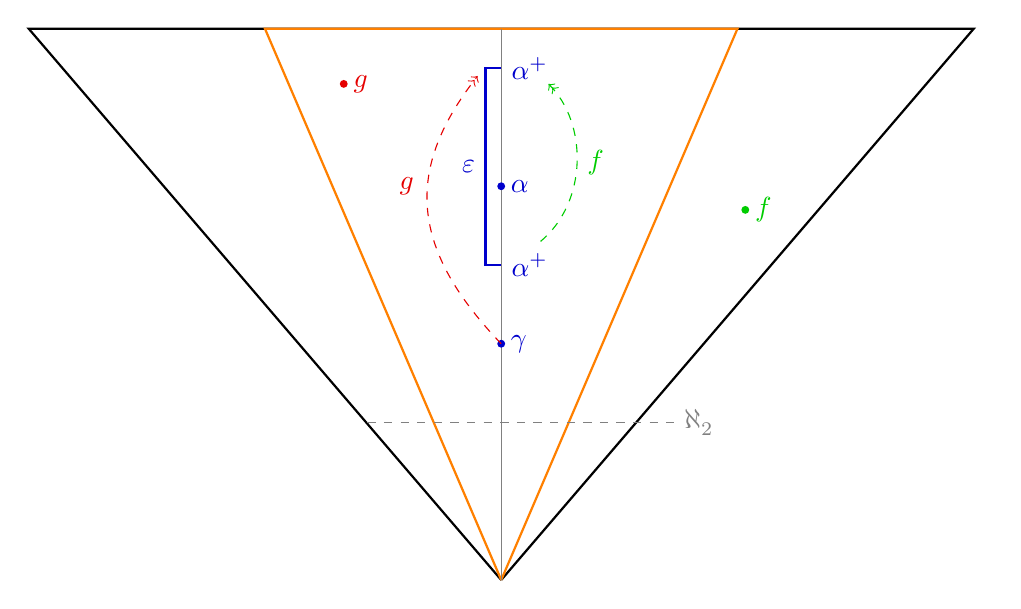
\begin{tikzpicture}

      % Borders
      \draw[black, thick] 
        (0, 0) 
        -- (-6, 7) 
        -- (6, 7) node[anchor=north west] {$\V$} 
        -- (0, 0);
      \draw[orange, thick] 
        (0, 0) 
        -- (-3, 7) 
        -- (3, 7) node[anchor=north west] {$\U$} 
        -- (0, 0);

      % Center line
      \draw[gray] 
        (0, 0) 
        -- (0, 7);

      % Aleph 2 line
      \draw[gray, dashed] 
        (-1.7, 2) 
        -- (2.2, 2) node[anchor=west] {$\aleph_2^{\V}$};

      % epsilon interval
      \draw[blue!80!black, thick] 
        (0, 4) node[anchor=west] {$\abs{\alpha^{+\U}}^{\V}$} 
        -- (-0.2, 4) 
        -- (-0.2, 5.25) node[anchor=east] {$\varepsilon$} 
        -- (-0.2, 6.5) 
        -- (0, 6.5) node[anchor=west] {$\alpha^{+\U}$};

      % alpha
      \fill[blue!80!black]
        (0, 5) circle (0.05cm) node[anchor=west] {$\alpha$};

      % gamma
      \fill[blue!80!black]
        (0, 3) circle (0.05cm) node[anchor=west] {$\gamma$};

       % g function
      \fill[red!90!black] 
        (-2, 6.3) node[anchor=west] {$g$} circle (0.05cm);
      \draw[red!90!black]
        (-1.2, 5) node {$g$};
      \draw[red!90!black, dashed, ->>]
        (0, 3) .. controls (-1.2, 4.25) and (-1.2, 5.25) .. (-0.3, 6.4);
      
       % f function
      \fill[green!80!black] 
        (3.1, 4.7) node[anchor=west] {$f$} circle (0.05cm);
      \draw[green!80!black]
        (1.2, 5.3) node {$f$};
      \draw[green!80!black, dashed, ->>]
        (0.5, 4.3) .. controls (1.1, 4.8) and (1.1, 5.8) .. (0.6, 6.3);

    \end{tikzpicture}
    \caption{Weak covering property}
  \end{figure}
\end{center}

\qquad When it comes to $(ii)$ we have to define what we mean by ``resembling $L$''. Ultimately this boils down to the current working definition of a \textit{mouse} and is still a work in progress. If our universe is no more complex than the strength of a Woodin cardinal however, then we know what the correct definition of a mouse is, and hence also what ``resembling $L$'' would mean in this context. The definition of mice along with the assumption of covering then turns out to imply that the core model will indeed inherit the large cardinal strength of the universe\footnote{To show this one first uses covering to show that $K$ is \textit{universal}, i.e. that it wins every coiteration. With universality at hand, a comparison argument with any $L[\vec E]$-model containing a large cardinal will then show that $K$ will have an inner model with the large cardinal in question.}.

\qquad To construct the core model one could then take a bottom-up approach, starting with $L$ and then carefully include the complexity of the universe while remaining similar to $L$\footnote{This strategy has a long history and current leading figures following it are Steel and Sargsyan.}. Alternatively, a top-down approach would be to define a structure which has \textit{all} the complexity of the universe, and then showing that this structure indeed exhibits these $L$-like properties\footnote{Woodin is pursuing this path.}.

\subsection{Constructing $K$}

The standard construction of $K$ takes the bottom-up approach. The first step towards this is the construction of $K^c$,\footnote{The ``c'' stands for \textit{certified}, as the extenders we put on the sequence was historically called \textit{certified extenders}.} which we build by recursion on the ordinals. We start with $K^c_0 := \emptyset$ and at every successor ordinal $\alpha$ we do one of two things:

\begin{enumerate}
  \item If there exists a ``nice'' extender indexed at $\alpha$ then we put it onto the extender sequence of $\core(K^c_\alpha$), where $\core(X)$ is the transitive collapse of a certain hull of $X$;\footnote{Think of $\core(X)$ as ``removing the noise of $X$''.}
  \item Otherwise we let $K^c_\alpha := \J(\core(K^c_{\alpha-1}))$, with $\J(x):=\text{rud}(\trcl(x\cup\{x\}))$ being the usual operator we use to build $L$ with Jensen's hierarchy.\\
\end{enumerate}

In other words, we are essentially building $L$ with extenders attached onto it in a canonical fashion. Taking cores at every step will ensure that the initial segments will be \textit{sound}, which ultimately is what guarantees iterability of $K^c$. The fact that we put on all the relevant extenders from $V$ is what will ensure the covering property of the model. It turns out that $K^c$ is not exactly what we want however, as it relies \textit{too much} on the surrounding universe, in contrast with $L$ whose construction procedure builds the exact same model in every universe. To attain this \textit{canonicity} we are again taking certain ``thick'' hulls of $K^c$ (again, think of it as removing the noise). The resulting construction \textit{almost} gives us what we want and is dubbed \textit{pseudo-K}. The problem with this is that the technicalities of the construction uses certain properties of a fixed cardinal $\Omega$, so to build the true core model we ``glue'' these pseudo-K's together.

\qquad The takeaway here is that whenever we are working with an initial segment of $K$ then that segment will be built using the recursive steps $(i)$ and $(ii)$ above, carefully including extenders from $V$. For more details, see \cite{JensenSteel} or \cite{MSc}.

\subsection{Properties of $K$}

In terms of applications of core model theory, the properties of $K$ are usually what matters. We touched on the weak covering property above, but for completeness we state most of the properties usually employed when working with $K$. In \cite{JensenSteel} they isolate a set of properties of $K$ which leads them to \textit{define} $K$ as the structure satisfying the conjunction of these properties. These are as follows.\footnote{See \cite{steel2010outline} for definitions of premice, iteration trees and iteration strategies.}

\begin{enumerate}
  \item $K$ is a transitive proper class premouse satisfying \zfc;
  \item $K$ is $\Sigma_2$-definable;
  \item $K$ has a $\Sigma_2$-definable iteration strategy $\Sigma$;
  \item $K$ is \textbf{generically absolute}, meaning that $K^V=K^{V[g]}$ and $\Sigma^{V[g]}\restr V=\Sigma^V$ for any $V$-generic filter $g\subset\mathbb P$ for a set-sized forcing notion $\mathbb P$;
  \item $K$ is \textbf{inductively defined}, meaning that $K\l\omega_1^V$ is $\Sigma_1$-definable over $J_{\omega_1}(\mathbb R)$;
  \item $K$ satisfies \textbf{weak covering} as in Definition \ref{defi.weak-covering}.\\
\end{enumerate}

On top of these properties, we will also employ the following property, which is proven in Lemmata 7.3.7--7.3.9 and 8.3.4 in \cite{Zeman}:

\qtheo[Zeman][theo.beaver]{
  Assume $0^\pistol$ does not exist. If $\mu$ is a countably complete weakly amenable $K$-measure then $\mu\in K$.
}

\subsection{Coiterations of mice}

One of the crucial lemmata in the theory of mice, of which $K$ is a special case, is the comparison lemma. Intuitively, it says that any two mice $\M,\N$ can be \textit{compared}, in the sense that we can transform $\M$ and $\N$ into new mice $\hat\M$ and $\hat\N$, respectively, such that either $\hat\M$ is an initial segment of $\hat\N$ or vice versa. Such a transformation is called a \textbf{coiteration}, which can be thought of as being successive applications of measures in the mice, forming iterative ultrapowers. For more details regarding mice and coiterations, see \cite{steel2010outline} or \cite{MSc}.

\lemm[Comparison lemma]{
  Let $\theta$ be an uncountable regular cardinal or $\theta=\on$. Let $\M$ and $\N$ be \textit{sound} mice of size $\leq\theta$. Then there are iterations $\T$ and $\U$ of $\M$ and $\N$ having last models $\hat\M$ and $\hat\N$, respectively, such that either
  \begin{enumerate}
    \item $\hat\M\init\hat\N$ and there is an elementary embedding $\pi\colon\M\to\hat\M$; or
    \item $\hat\N\init\hat\M$ and there is an elementary embedding $\pi\colon\N\to\hat\N$.$\hfill\qed$
  \end{enumerate}
}

\section{Forcing lemmata}
\label{prelims.forcing}

In this section we will cover a few results that we will need when working with elementary embeddings in different forcing extensions. These are the \textit{lifting criterion}, which characterises when we can lift an elementary embedding to a forcing extension, \textit{countable embedding absoluteness}, which allows us to ``transfer'' elementary embeddings from one forcing extension to another, and lastly a result that gives a sufficient condition for preserving sequence closure when moving to generic extensions.

\subsection{Lifting criterion}
When we are working with an elementary embedding $\pi\colon\M\to\N$ between sets in the universe, we would sometimes like to lift such an embedding to a generic extension, meaning that given a forcing notion $\mathbb P\in\M$ and an $\M$-generic $g\subset\mathbb P$, we are interested in when we can lift $\pi$ to an embedding
\eq{
  \pi^+\colon\M[g]\to\N[h],
}

where $h\subset\pi(\mathbb P)$ is $\N$-generic. The \textbf{lifting criterion} shows exactly when this is possible.

\prop[The Lifting Criterion; \cite{handbook-cummings} 9.1][prop.lifting-criterion]{
  Let $\pi\colon\M\to\N$ be an elementary embedding between weak $\kappa$-models. Fix a forcing notion $\mathbb P\in\M$, an $\M$-generic $g\subset\mathbb P$ and an $\N$-generic $h\subset\pi(\mathbb P)$. Then the following are equivalent:
  \begin{enumerate}
    \item $\pi[g]\subset h$;
    \item There exists an elementary $\pi^+\colon\M[g]\to\N[h]$ such that $\pi^+(g)=h$ and $\pi^+\restr\M = \pi$.
  \end{enumerate}
}
\proof{
  $(ii)\Rightarrow(i)$ is clear, so assume $(i)$. Define $\pi^+\colon\M[g]\to\N[h]$ as $\pi^+(\dot\tau^g) := \pi(\tau)^h$. To see that $\pi^+$ is well-defined fix $\dot\sigma,\dot\tau\in\M^{\mathbb P}$ such that $\dot\sigma^g=\dot\tau^g$, and fix $p\in g$ such that $p\forces\dot\sigma=\dot\tau$. By elementarity $\pi(p)\forces\pi(\dot\sigma)=\pi(\dot\tau)$, so since $\pi(p)\in h$ by $(i)$ we get that $\pi(\dot\sigma)^h=\pi(\dot\tau)^h$.

  \qquad To show elementarity, note that for $x\in\M$ it holds that $\pi(\check x) = \check{\pi(x)}$, implying $\pi^+(x)=\pi^+(\check x^g) = \pi(\check x)^h = \pi(x)$. Further, letting $\dot g\in\M^{\mathbb P}$ be the standard $\mathbb P$-name for $g$, then $\pi(\dot g)$ is the standard $\pi(\mathbb P)$-name for $h$ and therefore $\pi^+(g)=h$.
}

\subsection{Countable embedding absoluteness}
A key folklore lemma which we will frequently need when dealing with elementary embeddings existing in generic extensions is the following:

\lemm[Countable Embedding Absoluteness][lemm.ctblabs]{
  Let $\M,\N$ be sets, $\P$ a transitive class with $\M,\N\in\P$, and let $\pi\colon\M\to\N$ be an elementary embedding. Assume that $\P\models\zf^-+\dc+\godel{\text{$\M$ is countable}}$ and fix any finite $X\subset\M$.
  
  \qquad Then $\P$ contains an elementary embedding $\pi^*\colon\M\to\N$ which agrees with $\pi$ on $X$. If $\pi$ has a critical point and if $\M$ is transitive then we can also assume that $\crit\pi=\crit\pi^*$.\footnote{We are using transitivity of $\M$ to ensure that the \textit{ordinal} $\crit\pi$ exists.}
}
\proof{
  Let $\{a_i\mid i<\omega\}\in\P$ be an enumeration of $\M$ and set
  \eq{
    \M\restr n:=\{a_i\mid i<n\}.
  }
  
  Then, in $\P$, build the tree $\T$ of all partial isomorphisms between $\M\restr n$ and $\N$ for $n<\omega$, agreeing with $\pi$ on $X$, ordered by extension. Then $\T$ is illfounded in $V$ by assumption, so it is also illfounded in $\P$ since $\P$ is transitive and $\P\models\zf^-+\dc$. The branch then gives us the embedding $\pi^*$, and if $\crit\pi$ exists then we can ensure that it agrees with $\pi$ on the critical point and finitely many values by adding these conditions to $\T$.
}

The following proposition is an almost immediate corollary of Countable Embedding Absoluteness:

\qprop[][prop.coll]{
    Let $\M$ and $\N$ be transitive models and assume that there is a generic elementary embedding $\pi:\M\to \N$. Then $V^{\col(\omega,\M)}$ has an elementary embedding $\pi^*:\M\to\N$ which agrees with $\pi$ on any desired finite set and has the same critical point if it exists.
}

\subsection{Preservation of sequence closure}
The following lemma is from \cite{lucke-schlicht-notes} and gives a useful condition on when sequence closure is preserved when moving to generic extensions:

\lemm[][lemm.lucke-schlicht]{
  Let $\lambda$ be an infinite cardinal, $\M\models\zf^-$ a transitive model, $\mathbb P\in\M$ a $\lambda^+$-cc forcing notion and $g\subset\mathbb P$ an $\M$-generic filter. Then $V\models{^\lambda}\M\subset\M$ implies that $V[g]\models{^\lambda}\M\subset\M$.
}
\proof{
  Work in $V[g]$. Let $c:=\bra{c_\alpha\mid\alpha<\lambda}$ be a $\lambda$-sequence such that $c_\alpha\in\M[g]$ for every $\alpha<\lambda$. Fix for every $\alpha<\lambda$ a $\mathbb P$-name $\dot c_\alpha$ such that $\dot c_\alpha^g=c_\alpha$. Also let $\dot a$ be a $\mathbb P$-name with $\dot a^g=\bra{\dot c_\alpha\mid\alpha<\lambda}$ and choose $p\in g$ such that $V\models\godel{p\forces\forall\alpha<\check\lambda\colon\dot a(\alpha)\in\M^{\mathbb P}}$.

  \qquad Now, working in $V$, there is for each $\alpha<\lambda$ a maximal antichain $A_\alpha$ below $p$ such that every $q\in A_\alpha$ decides $\dot a(\alpha)$; i.e., $q\forces\godel{\dot a(\alpha)=\check x}$ for some $x\in\M$. Define now
  \eq{
    \sigma := \{((\alpha,x),q)\mid\alpha\in\lambda\land q\in A_\alpha\land q\forces\godel{\dot a(\alpha)=\check x}\}.
  }

  Then $p\forces\godel{\sigma=\dot a}$. Note that $\abs{\sigma}\leq\lambda$, since $\abs{A_\alpha}\leq\lambda$ for each $\alpha<\lambda$. Thus $\sigma\in\M$. Now it holds that
  \eq{
    V[g]\models\godel{\bra{\dot c_\alpha\mid\alpha<\lambda}=\dot a^g=\sigma^g\in\M[g]},
  }
  
  and we can compute $c=\bra{c_\alpha\mid\alpha<\lambda}=\bra{\dot c_\alpha^g\mid\alpha<\lambda}$ from $\bra{\dot c_\alpha\mid\alpha<\lambda}$ and $g$, so $c\in\M[g]$ by Replacement.
}

%\section{Ideals}
%\label{prelims.ideals}
%
%\defi{
%  Let $I$ be an ideal on a nonempty set $Z$. Let
%  \begin{enumerate}
%    \item $I^{+} := \mathcal{P}(Z) \setminus I$,
%    \item for $a,b \in I^{+}$ let $a \sim_{I} b$ iff $a \Delta b \in I$,
%    \item $\mathcal{P}(Z)/I:=\P(Z)/{\sim_I}$ is the Boolean algebra with subset inclusion modulo $\sim_I$.
%  \end{enumerate}
%
%  We call $\P(Z)/I$ the 
%  \textbf{associated forcing} to $I$.
%}
%
%\defi{
%  If $I$ is an ideal on a cardinal $\kappa$ and $g\subset\P(\kappa)/I$ $V$-generic then $g$ is a $V$-ultrafilter on $\kappa$ in $V[g]$, so that we may take the  \textbf{generic ultrapower} $\ult(V,g)$.
%}
%
%\prop{
%  Let $I$ be an ideal on a cardinal $\kappa$. Then..
%  \begin{enumerate}
%    \item if $I$ is $\kappa$-complete then so is any generic ultrafilter;
%    \item if $I$ is normal then so is any generic ultrafilter.$\hfill\circ$
%    \end{enumerate}
%    \todo{define $\kappa$-complete and normal for an ideal. Add reference.}
%}
%
%\xdefi{
%  Let $\lambda$ be any cardinal. Then an ideal $I$ on a cardinal
%  $\kappa$ is...
%  \begin{itemize}
%  \item \textbf{precipitous} if the generic ultrapower is wellfounded;
%  \item \textbf{$\lambda$-saturated} if the associated forcing has the $\lambda$-chain condition;
%  \item \textbf{$\lambda$-dense} if the associated forcing has a dense subset of size $\lambda$.$\hfill\circ$
%  \end{itemize}
%}
%
%Note that $\lambda$-dense trivially implies $\lambda^+$-saturated. We will need the following facts about $\omega_2$-saturated ideals on $\omega_1$:
%
%\prop[][prop.ideal]{
%  Let $I$ be an $\omega_2$-saturated ideal on $\omega_1$. Then $I$ is precipitous, and letting $j \colon V\to M$ be the generic ultrapower map, it holds that\todo{Parts (ii)-(v) is Example 4.29 in Foreman's handbook chapter. Perhaps include the proof.}
%  \begin{enumerate}
%    \item $M$ is closed under $\omega$-sequences in $V[g]$;
%    \item $j(\omega_1^V)=\omega_2^V=\omega_1^{V[g]}$;
%    \item $j(\omega_2^V)\in(\omega_2^V,\omega_3^V)$;
%    \item $j$ is continuous at $\omega_2^V$;
%    \item $j(\omega_n^V)=\omega_n^V=\omega_{n-1}^{V[g]}$ for all
%      $n\in[3,\omega]$.$\hfill\circ$
%  \end{enumerate}
%}
%
%As for the density, we in particular need the following fact:
%
%\qprop{ 
%  Let $I$ be an $\omega_1$-dense ideal on $\omega_1$. Then the associated forcing is forcing equivalent to $\col(\omega,\omega_1)$, so in particular it is homogeneous.
%}
%
%\proof{
%  \cite[Proposition~10.20]{Kanamori}.
%}
%
%\section{Descriptive Set Theory}
%\label{prelims.descriptive-set-theory}
%
%\begin{convention}
%  We will be using the ``logician's reals'',
%  meaning that $\mathbb{R} := {^{\omega}\omega}$ with the product
%  topology, having the sets $\{x\in\mathbb R\mid x\supset s\}$ for
%  $s\in{^{<\omega}\omega}$ as a clopen basis.
%\end{convention}
%
%\defi{
%  Let $A, B \subset \mathbb{R}$. We say that \textbf{$A$ is Wadge
%    reducible to $B$} (in symbols
%  $A \le_{W} B$) iff there is some continuous
%  function $f \colon \mathbb{R} \to \mathbb{R}$ such that
%  \[
%    A = f^{-1}[B] := \{ a \in A \mid f(a) \in B \}.
%  \]
%  We write $A <_{W} B$ iff $A \le_{W} B$ and $B \not \le_{W} A$.
%}
%
%\rema{
%  $\mathbb{R}$ and $\mathbb{R}^{n}$, for $1 \leq n \le \omega$
%  are homeomorphic and we shall often identify them with one another.
%  
%}
%
%\defi{
%  Subseteq of $\mathcal{R}$ are called \textbf{pointsets}
%  . Subsets of $\mathcal{P}(\mathbb{R})$ are called
%  \textbf{pointclasses} .
%
%}
%
%\defi{
%  Let $\Gamma$ be a pointclass. We define
%  \begin{enumerate}
%  \item $\exists^{\mathbb{R}} \Gamma := \{ A \mid \exists B \in \Gamma \colon A = \{ x \in \mathbb{R} \mid \exists y \in \mathbb{R} (x,y) \in B \} \}$, 
%  \item
%    $\forall^{\mathbb{R}} \Gamma := \{ A \mid \exists B \in \Gamma
%    \colon A = \{ x \in \mathbb{R} \mid \forall y \in \mathbb{R} (x,y)
%    \in B \} \}$. \Gamma$}
%  \end{enumerate}
%}
%
%\defi{
%  Let $\Gamma$ be a pointclass. We define
%  \begin{enumerate}
%  \item
%    $\overset{\smallsmile}{\Gamma} := \{ \mathbb{R} \setminus A \mid A \in
%    \Gamma \}$ ,
%  \item $\Delta_{\Gamma} := \Gamma \cap \overset{\smallsmile}{\Gamma}$  and
%  \item $\underset{\sim}{\Gamma} := \exists^{\mathbb{R}} \Gamma$ .
%  \end{enumerate}
%}
%
%\begin{lemma}[\cite{Wadge}]
%  Assume $\zf + \ad$ and let $A, B \subset \mathbb{R}$. Then
%  \[
%    A \le_{W} B \text{ or } B \le_{W} \mathbb{R} \setminus A.
%  \]  
%\end{lemma}
%
%\begin{lemma}[Martin-Monk-Wadge]
%  Assume $\zf + \ad + \dc_{\mathbb{R}}$. Then
%  $\leq_{W}$ is wellfounded.\footnote{See \cite{Larson} for a proof.}
%\end{lemma}
%
%\begin{remark}
%  When considering $(\mathcal{P}(\mathbb{R}); \le_{W})$ in a
%  $\zf + \ad+\dc_{\mathbb R}$ context, we will often tacitly identify
%  $A \subset \mathbb{R}$ with its complement, making $<_W$ a wellorder.
%\end{remark}
%
%\defi[$\zf + \ad + \dc_{\mathbb{R}}$]{
%  Let $A \subset \mathbb{R}$. Then the \textbf{Wadge rank of $A$}
%  is defined recursively as
%  $\abs A_{W} := \sup\{\abs B_W+1\mid B <_W A\}$.  }
%
%\begin{definition}
%  Let $X$ be a set. We write $\od_{X}$ for the
%  collection of all $A$ for which there is some formula $\phi$,
%  ordinals $\alpha_{0}, \ldots, \alpha_{k}$ and $x_{0}, \ldots, x_{l}\in X$
%  with
%  \[
%    A = \{ a \mid \phi[a, \alpha_{0}, \ldots, \alpha_{k}, x_{0},
%    \ldots, x_{l}] \}.\tag*{$\circ$}
%  \]
%  We write $\hod_{X}$ for the collection of all $A$ such that
%  $\tc(\{A\}) \subset \od_{X}$. \\
%  If $X = \emptyset$, we will often drop the subscript and simply
%  write $\od$ and $\hod$ for $\od_{\emptyset}$ and $\hod_{\emptyset}$
%  respectively.
%\end{definition}
%
%\defi[$\zf + \ad + \dc_{\mathbb{R}}$]{ For $B \subset \mathbb{R}$
%  let \eq{
%    \theta_{B} :& = \sup \{ \abs A_{W} \mid \exists x \in
%    \mathbb{R} \colon A \in \od_{\mathbb{R} \cup \{B \}} \} \\
%    & = \sup \{ \alpha \in \on \mid \text{ there is a } \od_{\mathbb{R} \cup
%      \{B\}} \text{-surjection } f \colon \mathbb{R} \to \alpha \}.
%  }
%\todo{Verify that these two values are in fact identical.}
%}
%
%\defi[$\zf + \ad + \dc_{\mathbb{R}}$]{  Define
%  the \textbf{Solovay sequence}
%  $\bra{\theta_{\alpha} \mid \alpha \le \Omega}$
%   \mid \alpha \le \Omega)$}
%   as follows:
%  \begin{enumerate}
%  \item
%    $\theta_{0} := \theta_{\emptyset}$,
%  \item if there is some $B$ such that $|B|_{W} = \theta_{\alpha}$ let $\theta_{\alpha + 1} := \theta_{B}$.\footnote{Since
%        continuous functions are coded by reals, this is independent
%        of the choice of $B$.}
%  \item if $\alpha$ is a limit ordinal, we let
%    $\theta_{\alpha} := \sup_{\beta < \alpha} \theta_{\beta}$.
%  \end{enumerate}
%  Finally, $\Omega$ is the least ordinal such that
%  $\theta_{\alpha+1} = \theta_{\alpha}$, and
%  $\Theta := \theta_{\Omega}$.
%}

\end{document}
